\chapter{Основная часть}
\label{ch:chap1}


\section{Знакомство с основными задачами отдела программирования}

«Савушкин продукт» $-$ современное хорошо автоматизированное производство. Все программное обеспечение организация разрабатывает сама.
По результатам моего опроса сотрудников одними из задач, которые решаются посредством программирования являются:

\begin{itemize}
    \item Разработка программного обеспечения терминала сбора данных, включая на базе ОС Android.
    \begin{itemize}
        \item языки: C#, Kotlin
        \item среда разработки: Android Studio, Visual Studio (2008)
    \end{itemize}
    \item Автоматизация работы отдела продаж, реализация.
    \begin{itemize}
        \item языки: Kotlin
        \item среда разработки: Android Studio
    \end{itemize}
    \item Разработка инструмента реализации.
     \begin {itemize}
     \item языки: Delphi, Java, Python
     \item  среда разработки: Rad Studio
     \end{itemize}
  \item Разработка мобильного приложения для регистрации «претензий»
   \begin{itemize} 
       \item языки:  Kotlin, Java, Java Script
       \item среда разработки: Android Studio
   \end{itemize}
   \item Разработка программного обеспечения для отслеживания грузовых машин.
   \begin{itemize}
       \item языки: PHP, Java Script
       \item среда разработки: Visual Studio Code
   \end{itemize}
   \item Разработка, тестирование проекта систем вентиляции и кондиционирования.
   \begin{itemize}
       \item языки: Lua
       \item среда разработки: Visual Studio Code, Eplan Electric
   \end{itemize}
   \item Работа со SCADA Monitor системами, разработка проекта.
   \begin{itemize}
       \item языки: Delphi
   \end{itemize}
   \item Разработка программного обеспечения для работы с контроллерами.
   \begin{itemize}
       \item языки: C, C++
       \item среда разработки: Visual Studio
   \end{itemize}
   \item Разработка SCADA и системы маркировки.
   \begin{itemize}
       \item языки: Delphi, C++, C#, Python, SQL
       \item среда разработки: Visual Studio, Rad Studio
   \end{itemize}
   \item Автоматизация производства, реализация проектов.
   \begin{itemize}
      \item языки: Delphi, C++, C#, Python, SQL
      \item среда разработки: Clion, Rider, Visual Studio, VS Code
  \end{itemize}
  \item  Разработка дополнительного программного обеспечения к Eplan (ПО для проектирования электрических систем и автоматизации производства, позволяет создавать схемы, планировать расположение оборудования, генерировать список материалов и многое другое.)
  \begin{itemize}
      \item языки: C\#
      \item среда разработки: Visual Studio
  \end{itemize}
  \item Консультирование пользователей и программистов по работе с 1С, анализ работы 1С.
  \begin{itemize}
      \item языки: 1С
      \item среда разработки: 1С:Предприятие, 1C:Enterprise Development Tools
  \end{itemize}
  \item Работа, тестирование отчетов документов накладных, устранение системных неполадок, добавление нового функционала.
  \begin{itemize}
      \item языки: 1С
      \item среда разработки: 1С:Предприятие, 1C:Enterprise Development Tools
  \end{itemize}
\end{itemize}
В качестве системы контроля версий используется Git, иногда с графическом интерфейсом GitKraken.

В лаборатории «Савушкин продукт» на базе БрГТУ ведется работа над техническим зрением, которое позволяет автоматически отбраковывать некачественные товары, работа с роботами манипуляторами и контроллерами, а также рассматриваются перспективы и возможности внедрения электронных цен в магазины.

 \begin{figure}[ht]
	\centering
\hspace*{\fill}%
	\begin{subfigure}[b]{0.49\textwidth}
        \centering
		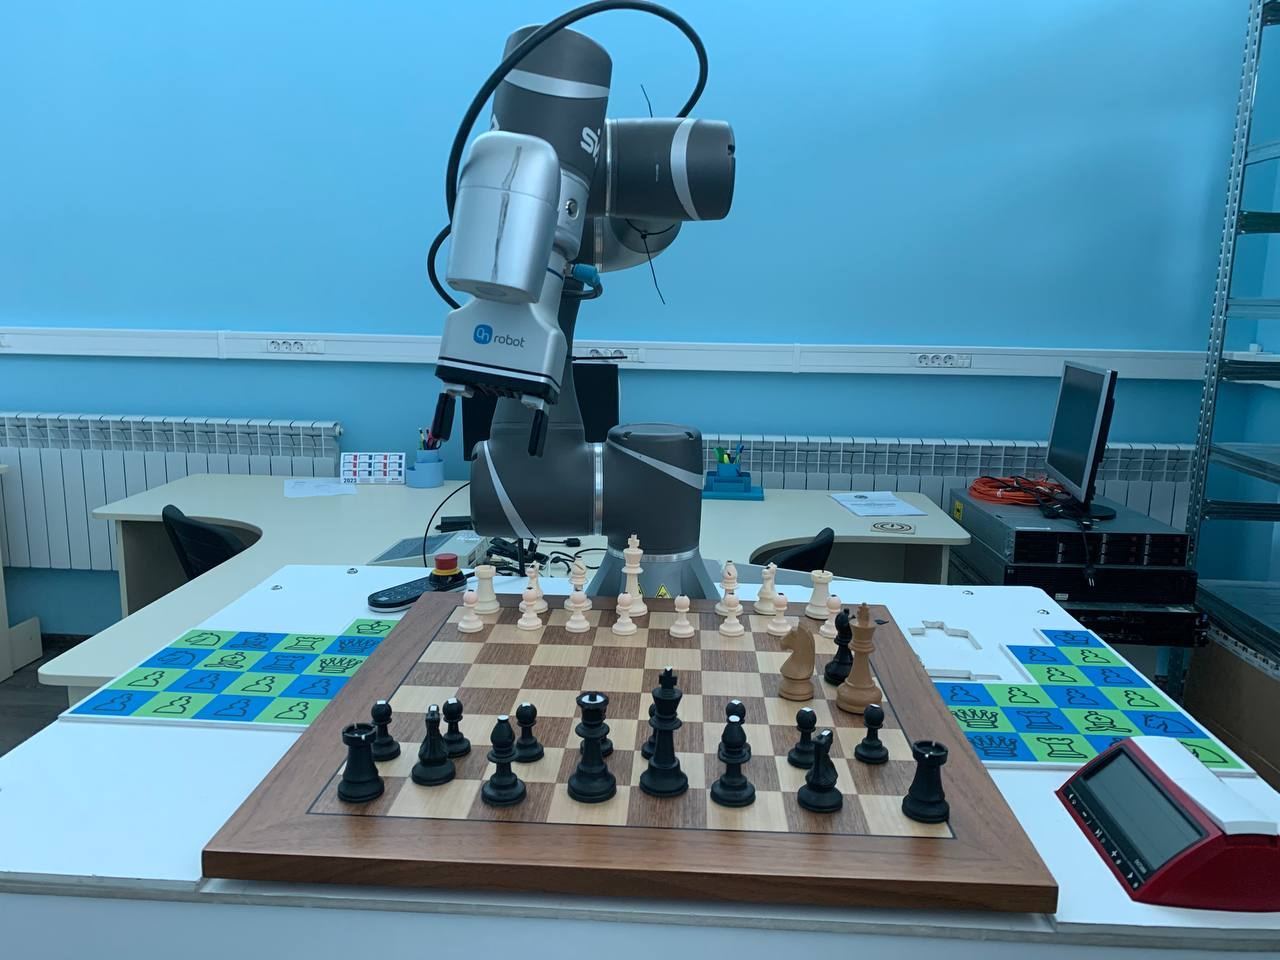
\includegraphics[height=5cm,keepaspectratio]{images/chess.jpg}
		\caption{}
		\label{fig:chess}
	\end{subfigure}
 \hfill
	\begin{subfigure}[b]{0.49\textwidth}
        \centering
		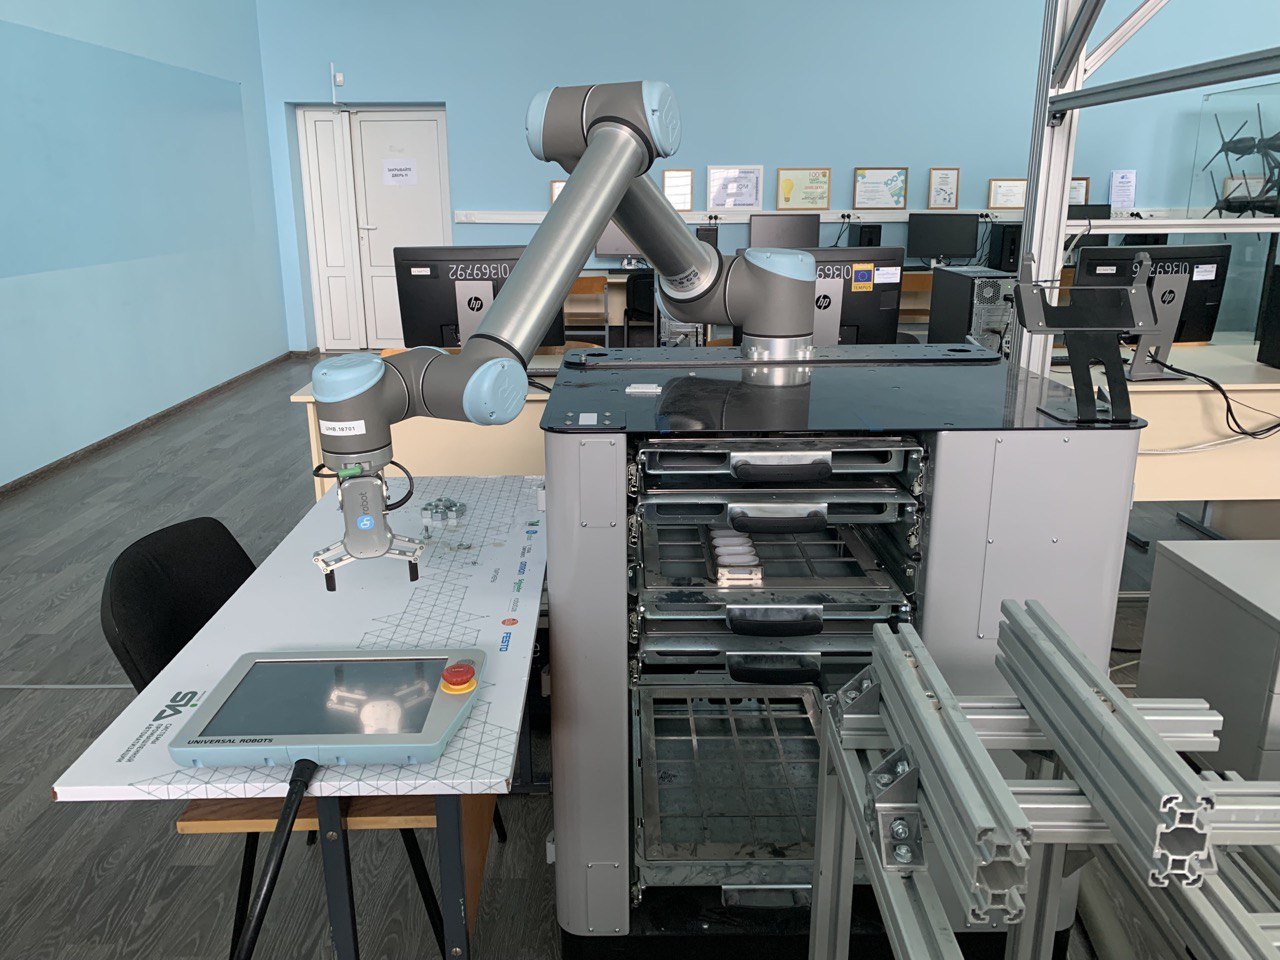
\includegraphics[height=5cm,keepaspectratio]{images/маншир.jpg}
        \caption{}
		\label{fig:маншир}
	\end{subfigure}
 \hspace*{\fill}%
	\begin{subfigure}[b]{0.49\textwidth}
        \centering
		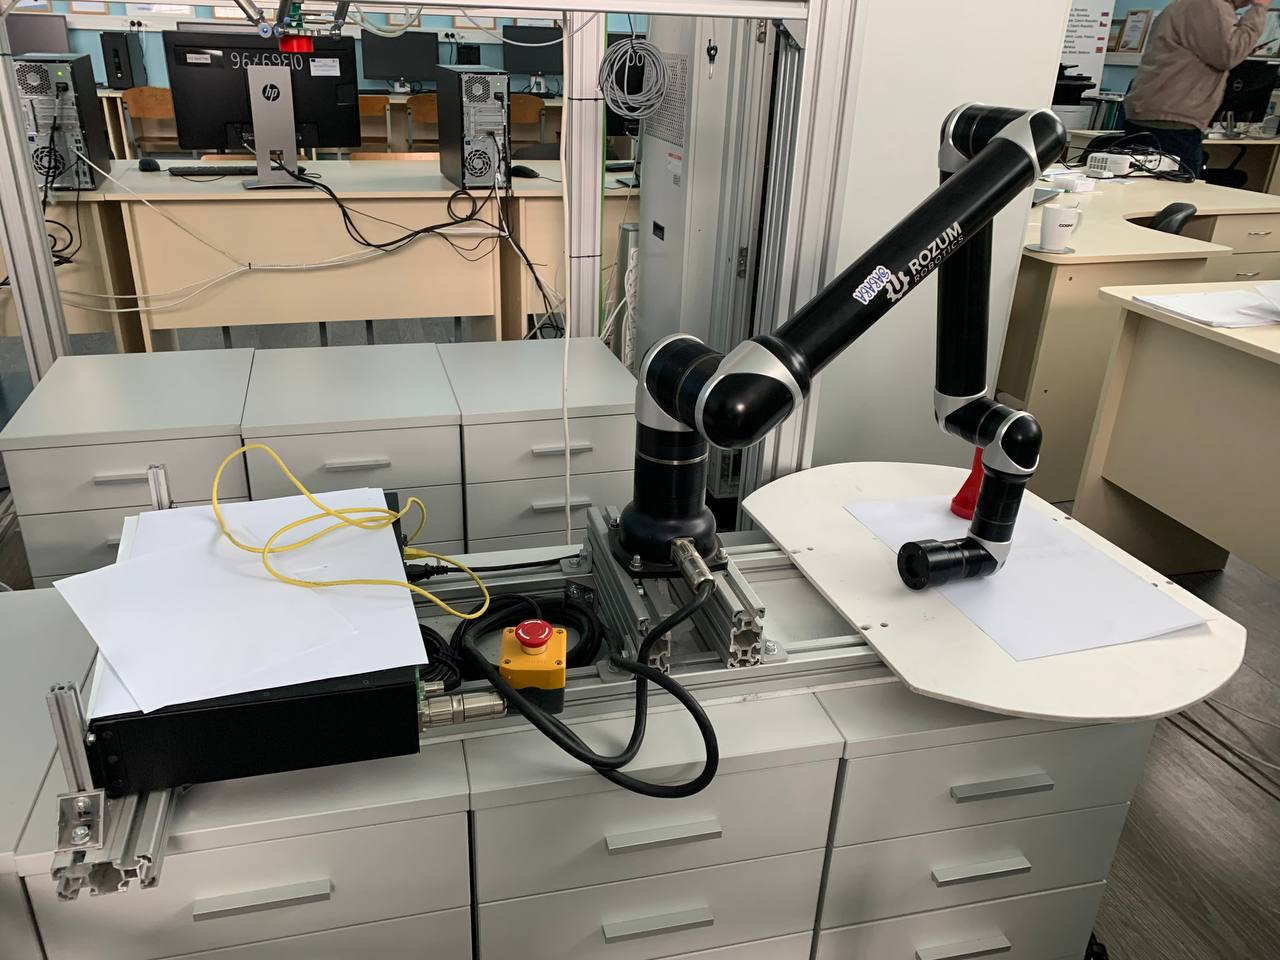
\includegraphics[height=5cm,keepaspectratio]{images/blr.jpg}
		\caption{}
		\label{fig:blr}
	\end{subfigure}
 \hfill
	\begin{subfigure}[b]{0.49\textwidth}
        \centering
		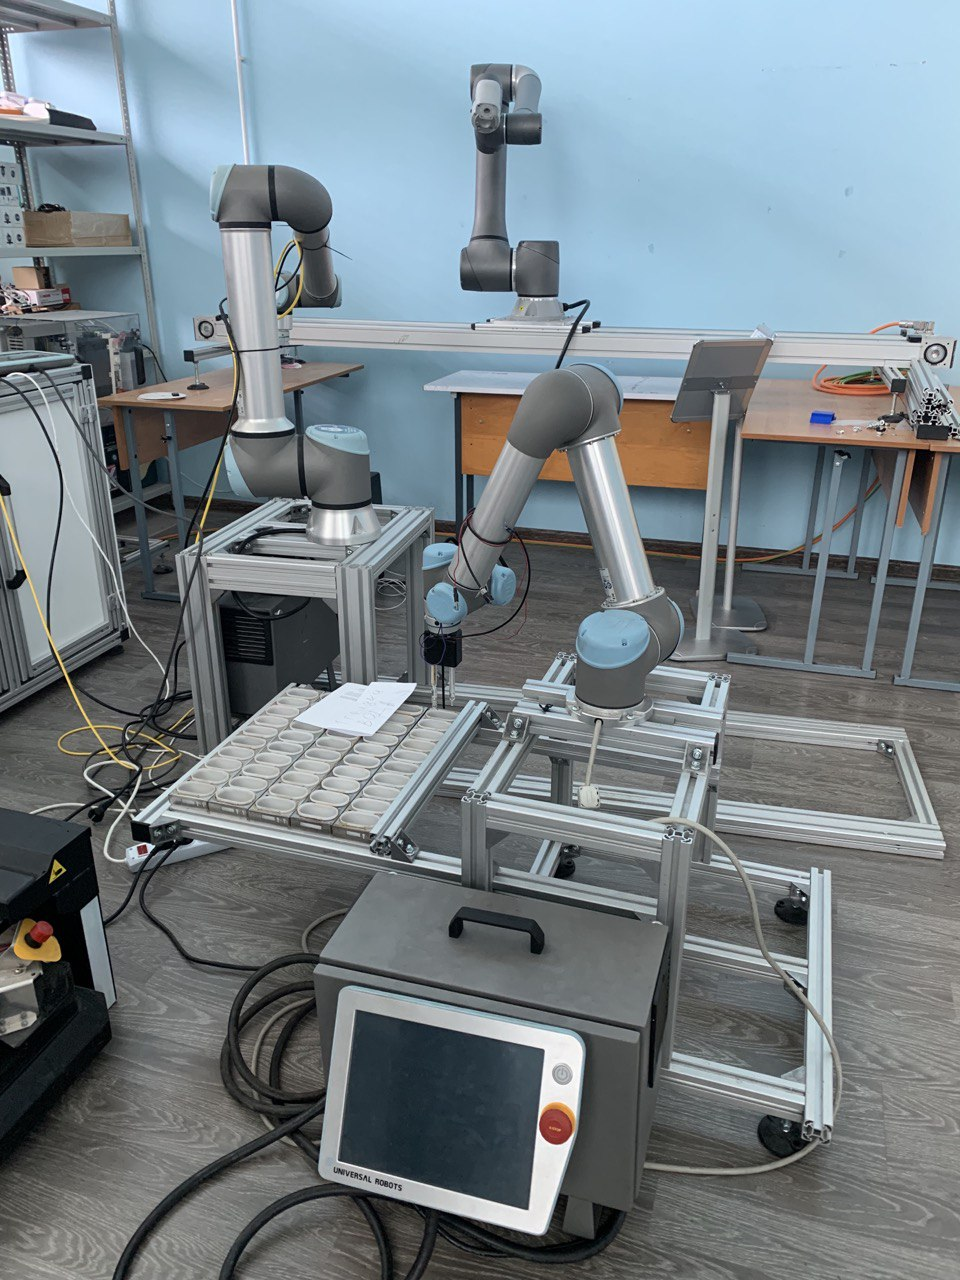
\includegraphics[height=5cm,keepaspectratio]{images/манипулятор.jpg}
        \caption{}
		\label{fig:манипулятор}
	\end{subfigure}

\hspace*{\fill}%
	\caption{Роботы манипуляторы. }
	\label{fig:robot}
 
\end{figure}
 \hfill


 \begin{figure}[ht]
 \centering
		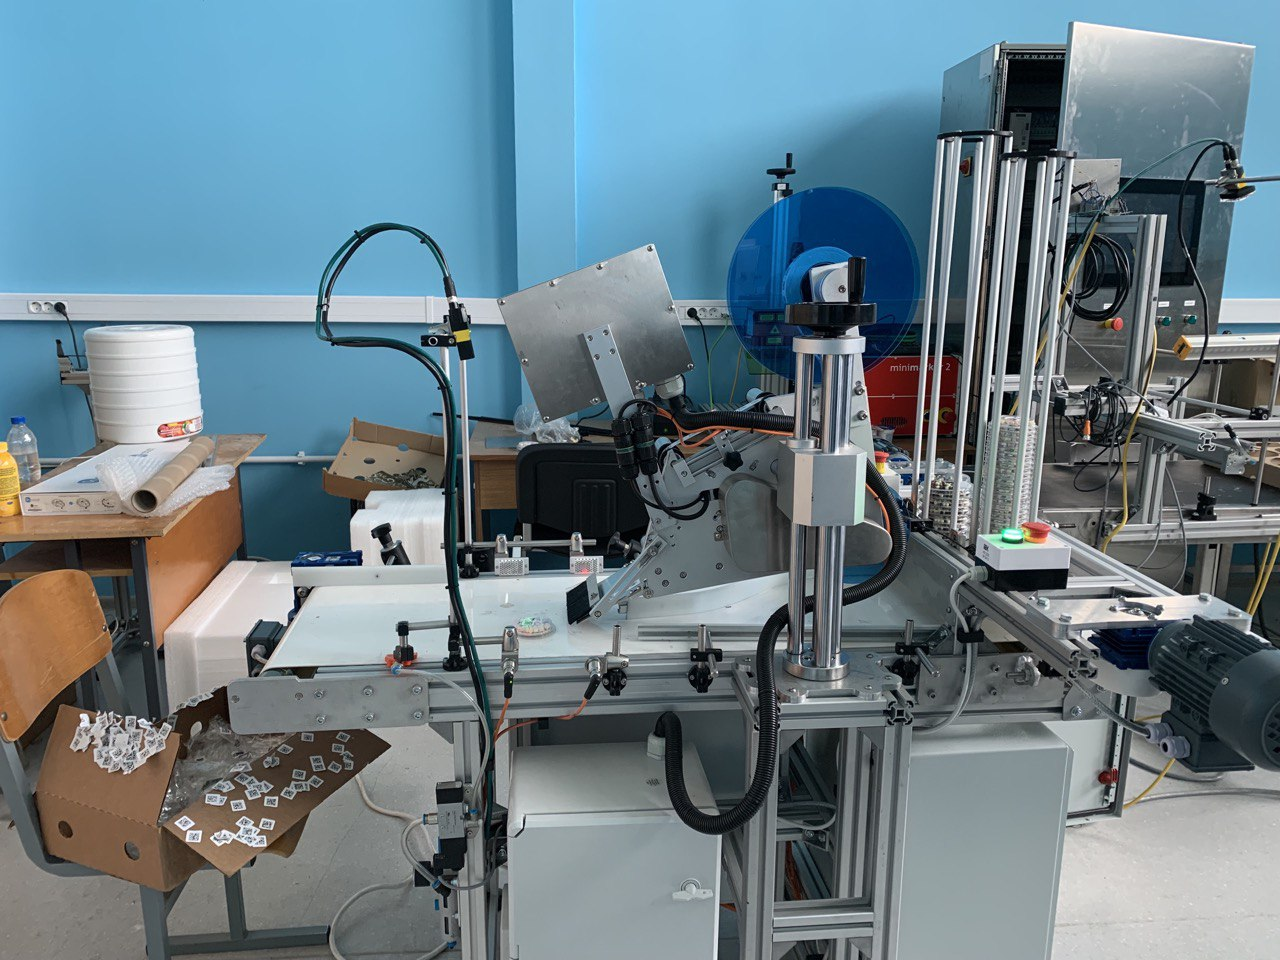
\includegraphics[height =10 cm, keepaspectratio]{images/техзрение.jpg}
		\caption{ Установка для работы с техническим зрением}
		\label{fig:техзрение}
	\end{figure}

\section{ Проделанная работа }

В ходе практики мне довелось заниматься сборкой и запуском проекта на контроллере исходники которого можно найти на GitHub \textcolor{blue}{savushkin-r-d/T1-PLCnext-Demo}, а также обновлением устаревшей документации с помощью Markdown. После запуска данная программа позволяла считывать данные с датчика температуры.
Моим главным заданием на практике было сделать симуляцию датчика температуры при запуске проекта  \textcolor{blue}{savushkin-r-d/ptusa\_main} в режиме эмуляции. То есть программа должна делать вид, что она подключена к контроллеру и считывает данные температуры. Значения температуры должны соответствовать нормальному распределению.

\begin{figure}[ht]
 \centering
		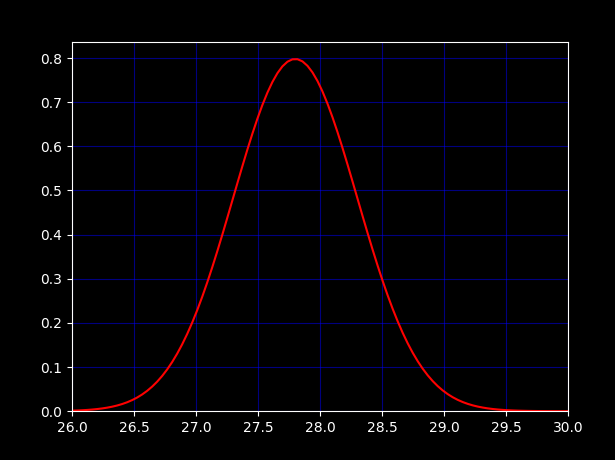
\includegraphics[height =10 cm, keepaspectratio]{images/normal.png}
		\caption{ График функции нормального распределения}
		\label{fig:normal}
	\end{figure}

Для этого мне нужно было разобраться в иерархии классов проекта \textcolor{blue}{ptusa\_main}, изменить функцию получения значений температуры \textcolor{teal}{get\_value()}, написать свой класс \textcolor{teal}{analog\_emulator}, ответственный за возврат значений аналоговых устройств в режиме эмуляции, у которого есть собственный метод \textcolor{teal}{get\_value()}, а затем все это протестировать средствами \textcolor{blue}{googletest} и \textcolor{blue}{github actions}. Все это делолось на языке программирования C++, 11 стандарта. Проект кроссплатформенный и собирается на CMake. Генерацией чисел, которые соответствуют нормальному распределению занималась функция STL \textcolor{teal}{std::normal\_distribution}. Данной функции передаются в качестве параметров мат. ожидание и стандартное отклонение, в программе предусмотрена возможность также в дальнейшем модифицировать эти параметры. Более подробно все изложено в написанном мною {\textcolor{blue}{user\_manual}, Это краткая документация к моему заданию. 

В тестах проверялась правильность инициализации членов класса в конструкторе, работа метода для модификации параметров  в \textcolor{teal}{std::normal\_distribution}.
